\pagebreak
\section{Results and Discussion}
\subsection{French}
\label{sec:results}

In this section we provide some of the most relevant results we got during the development phase.
We are considering five principal milestones that, within many different trials, led us to improve significantly our \ac{MAP} score and the overall number of relevant documents actually retrieved.


    \begin{table}[h]
    \centering
    \begin{tabular}{ |l|c|c|c|c|c| }
        \hline
        metric & run1 & run2  & run3 & run4 &run 5 \\ \hline
        num\_q & 663 & 663 & 669 & 669 & 667 \\ \hline
        num\_ret & 654909 & 655684 & 658446 & 658347 & 657903 \\ \hline
        num\_rel & 2571 & 2571 & 2611 & 2611 & 2600 \\ \hline
        num\_rel\_ret & 1914 & 2084 & 2182 & 2191 & 2232 \\ \hline
        map & 0.1553 & 0.1875 & 0.2022 & 0.2029 & 0.2351 \\ \hline
        gm\_map & 0.0178 & 0.0348 & 0.046 & 0.0459 & 0.0629 \\ \hline
        Rprec & 0.1276 & 0.1571 & 0.1697 & 0.1628 & 0.2022 \\ \hline
        bpref & 0.3331 & 0.3626 & 0.3734 & 0.3761 & 0.3861 \\ \hline
        recip\_rank & 0.261 & 0.3037 & 0.3287 & 0.3281 & 0.3945 \\ \hline
        iprec\_at\_recall\_0.00 & 0.2775 & 0.3242 & 0.3499 & 0.3526 & 0.4182 \\ \hline
        iprec\_at\_recall\_0.10 & 0.2771 & 0.3236 & 0.3494 & 0.3523 & 0.4175 \\ \hline
        iprec\_at\_recall\_0.20 & 0.2577 & 0.3076 & 0.3324 & 0.337 & 0.3927 \\ \hline
        iprec\_at\_recall\_0.30 & 0.2113 & 0.2523 & 0.2679 & 0.2743 & 0.3236 \\ \hline
        iprec\_at\_recall\_0.40 & 0.1732 & 0.2152 & 0.2316 & 0.2323 & 0.2716 \\ \hline
        iprec\_at\_recall\_0.50 & 0.1614 & 0.2036 & 0.2193 & 0.2192 & 0.2533 \\ \hline
        iprec\_at\_recall\_0.60 & 0.133 & 0.1636 & 0.1786 & 0.1758 & 0.2014 \\ \hline
        iprec\_at\_recall\_0.70 & 0.1061 & 0.1281 & 0.1402 & 0.1402 & 0.1552 \\ \hline
        iprec\_at\_recall\_0.80 & 0.0892 & 0.1091 & 0.1178 & 0.12 & 0.1295 \\ \hline
        iprec\_at\_recall\_0.90 & 0.0742 & 0.0896 & 0.0956 & 0.0992 & 0.1033 \\ \hline
        iprec\_at\_recall\_1.00 & 0.0741 & 0.0895 & 0.0954 & 0.0986 & 0.1028 \\ \hline
        P\_5 & 0.1222 & 0.1475 & 0.1599 & 0.1614 & 0.1874 \\ \hline
        P\_10 & 0.0973 & 0.1192 & 0.1296 & 0.1312 & 0.1432 \\ \hline
        P\_15 & 0.0797 & 0.0965 & 0.1049 & 0.1068 & 0.1135 \\ \hline
        P\_20 & 0.0668 & 0.0805 & 0.088 & 0.0891 & 0.0935 \\ \hline
        P\_30 & 0.0519 & 0.0616 & 0.0661 & 0.0668 & 0.0703 \\ \hline
        P\_100 & 0.0206 & 0.0236 & 0.0256 & 0.0258 & 0.0268 \\ \hline
        P\_200 & 0.0116 & 0.0132 & 0.014 & 0.0141 & 0.0148 \\ \hline
        P\_500 & 0.0053 & 0.0059 & 0.0061 & 0.0061 & 0.0064 \\ \hline
        P\_1000 & 0.0029 & 0.0031 & 0.0033 & 0.0033 & 0.0033 \\ \hline
    \end{tabular}

\end{table}


\begin{figure}[h!]
    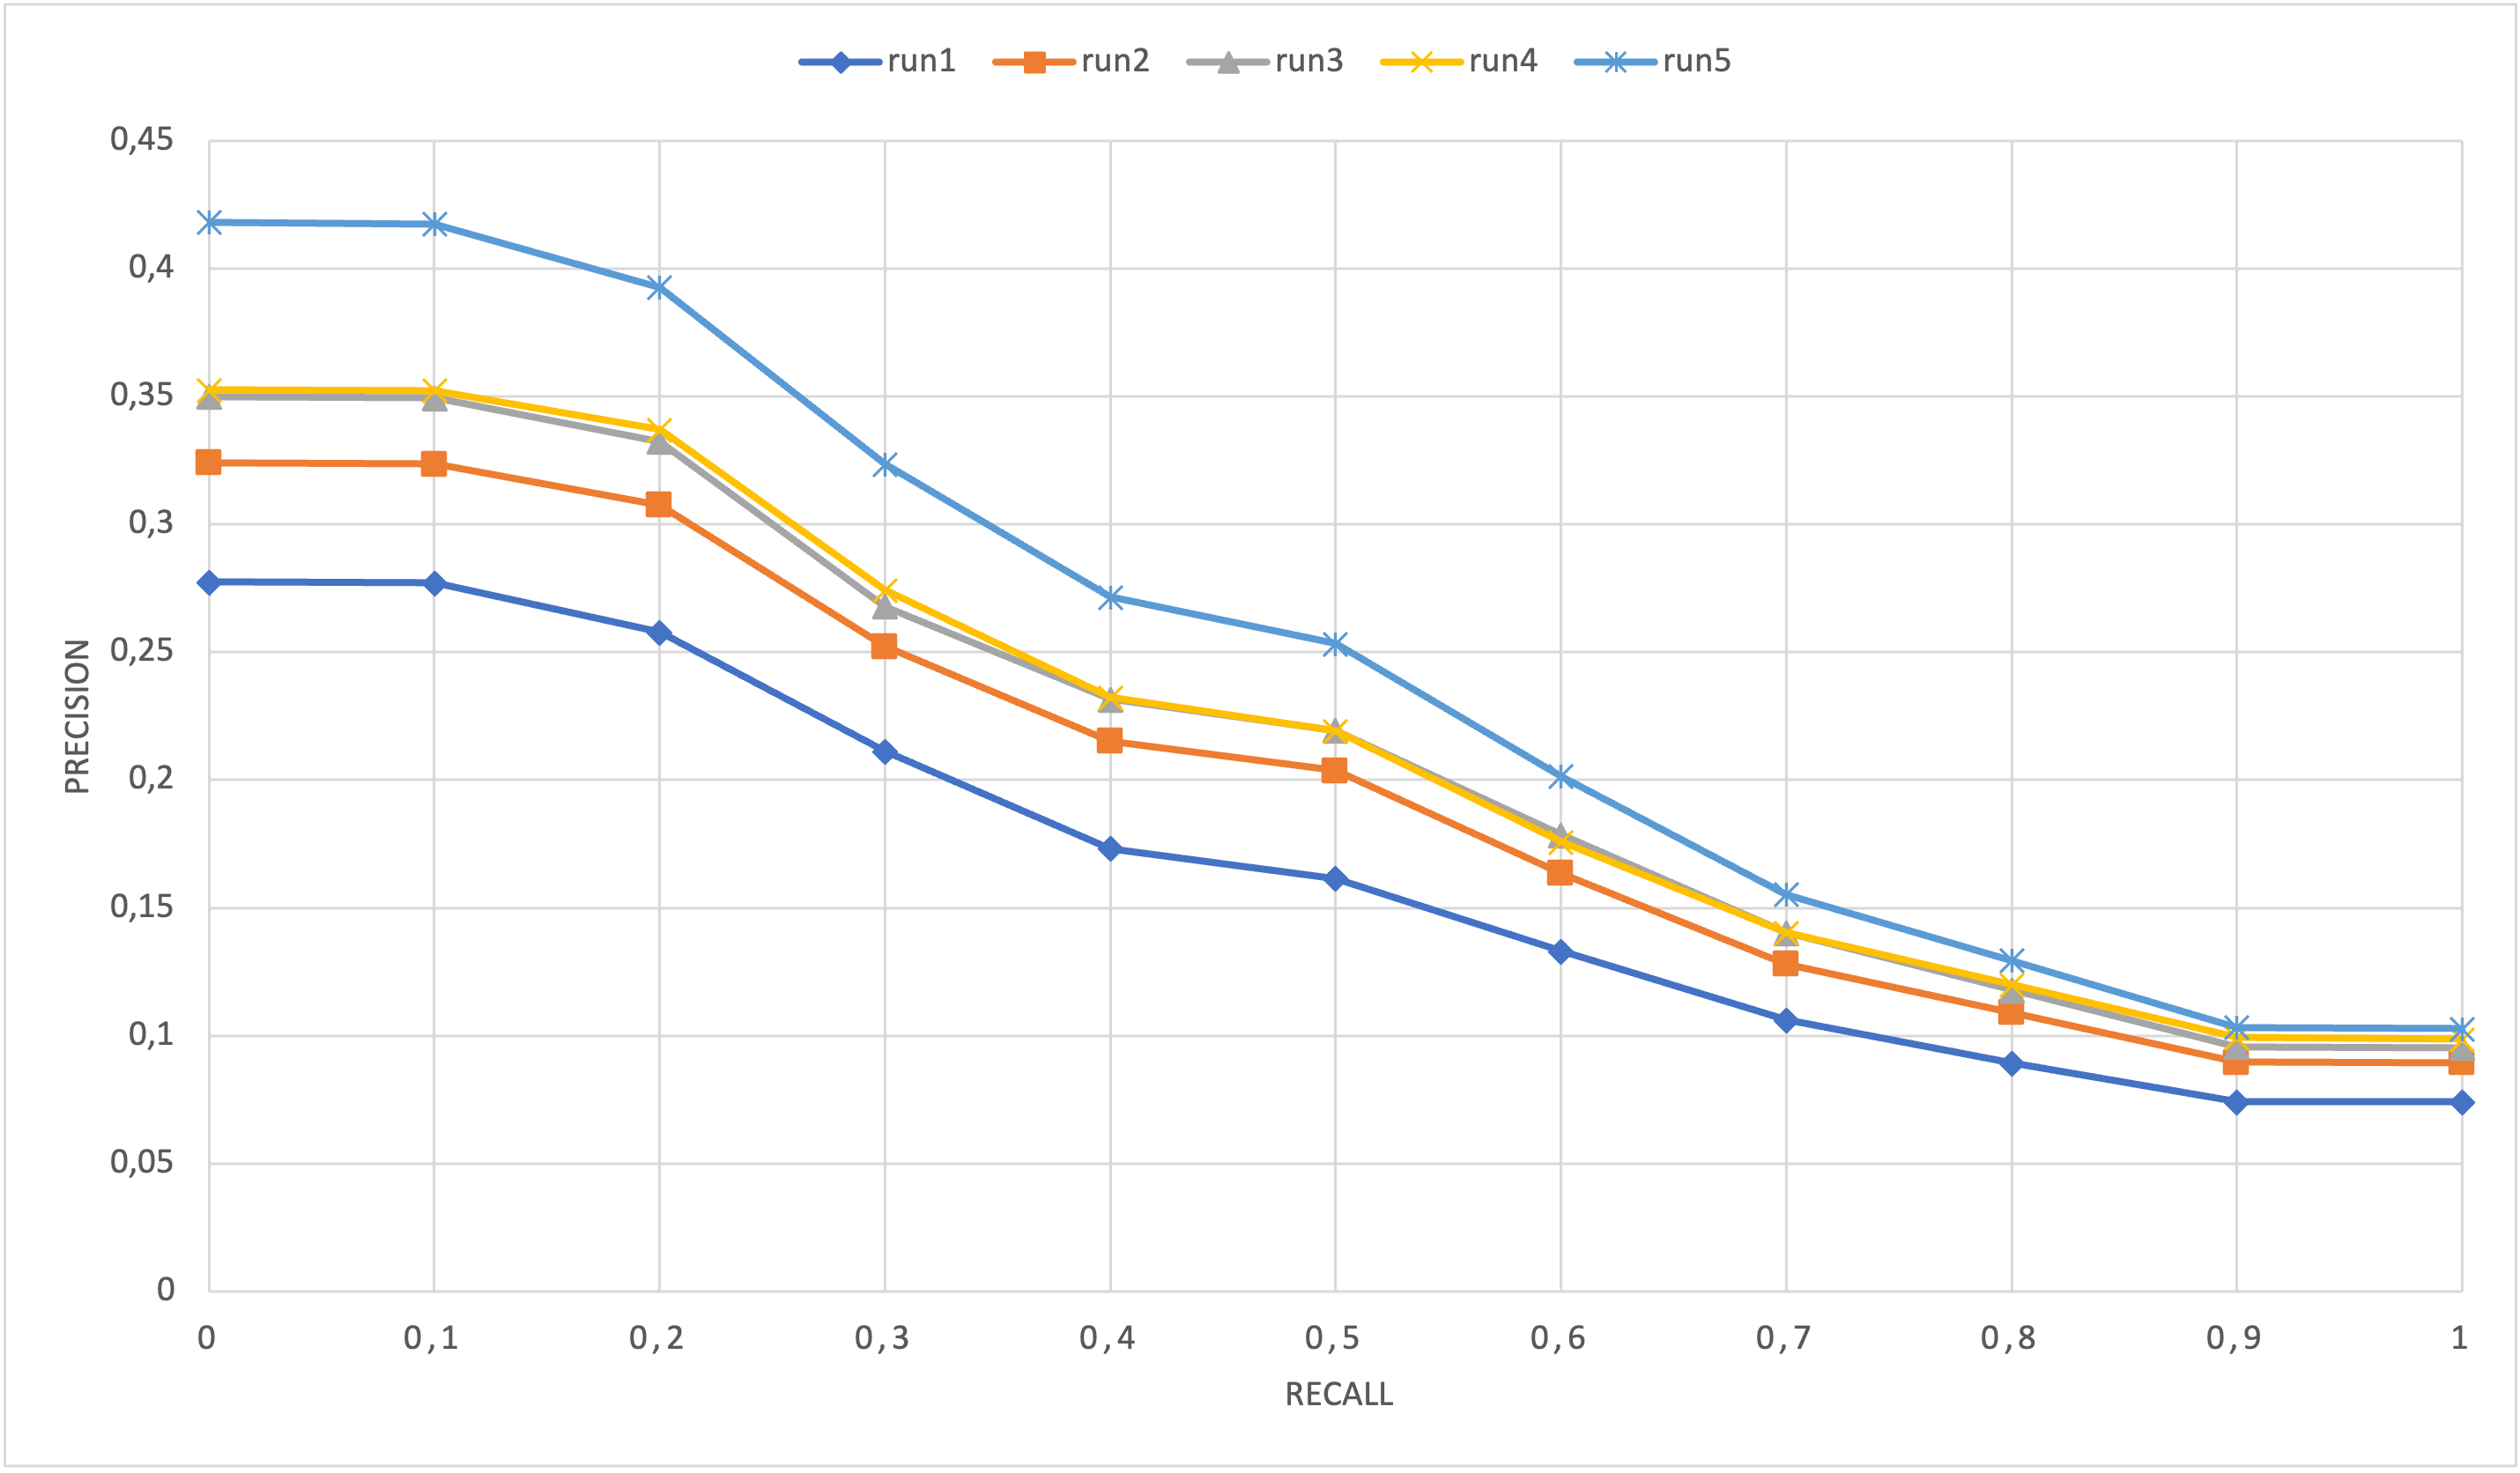
\includegraphics[width=\textwidth]{figure/rp_french.png}
    \caption{Recall and precision graph}
    \label{fig:rp_french}
\end{figure}

First of all, given that we were provided with two different version of the same document's \textit{corpora}, our first idea was to try with the English version.\\ 
We noticed that the best combination of basic \ac{IR} tools were to use the \textit{Porter} stemmer, a lenght filter from 1 to 10, and a list of stopword composed by some standard terms and more from the top 600 extracted from the index.
The very first big milestone, that helped us to increment the \ac{MAP} of around +3.5\%, was the \textit{JavaScript} code cleaner, since we noticed by inspection that many documents were having these type of scripts inside.\\
Always by inspecting some documents and queries, and also considering that the original collection was the French version (translated then in English), we observed that the translation was very poor: by switching to French
with just cleaning the \textit{JS} code and some other minor cleaning tools, without even using an adequate stoplist and a correct stemmer for the French language, the \ac{MAP} was increasing by +5\%. \\
2 more points were achieved with a stop list built for French in the same way we did previously for English, the \textit{FrenchLightStemFilter} \cite{solrfrenchlightstemfilter} as stemmer, and moving the lenght filter from 2 to 15 (as we noticed French tends to have longer words). \\
We tried some \ac{NLP} techniques for English, in particular using \ac{POS} techniques, to see if there were improvements, and in case apply it to our main implementation for French with an appropriate model, but results 
were not interesting, and also the computing time was definitely too costly.
Another approach we tried and that carried an improvement was to use \textit{Query expansion}: first we used some generative text models to expand our queries, then we decided to weight different query scores by boosting the original one linearly with respect to the number
%of expansion used, and without boosting the expansion: this carried to us an extra MAP point.
of expansion used. This made us gain an extra \ac{MAP} point.
\newline
We try to generate the embeddings for each document based on word2vector, we use pre-trained word2vec model \textit{frWac\_no\_postag\_no\_phrase\_500\_cbow\_cut100}~\cite{fauconnier_2015} for French. Then we calculate the embedding for each document and index them as KnnFloatVectorField in lucene and use KnnFloatVectorQuery for searching the query to find the k nearest documents to the target vector according to the vectors in the given field, but the results (overall map ~0.08) are not satisfying us and everything goes worser than the case of indexing and searching without anything.
We tried to combine different similarities rather than using the classic \textit{BM25Similarity}: we tried to use the Lucene \textit{MultiSimilarity} \cite{lucenemultisimilarity}, that allows to combine equally the score of two or more similarity scores, but it does not allow to
tune the weights. Then, we tried to reimplement the \textit{MultiSimilarity} class with tuning options, but results were always lower than the standard \textit{BM25Similarity}. Some minor improvements came up by fine tuning the document-length
normalization \textit{b} parameter and the term frequency component \textit{k1} parameter of the \textit{BM25Similarity}.
The last main implementation we did was to use some \textit{Re-ranking} techniques: TODO (?) 
Lastly, some minor addings were setted on the \textit{Analyzer} (\cite{analyzer_subsec}) by implementing the Lucene \textit{ElisionFilter} (for French) \cite{luceneelisionfilter}, that aims to remove apostrophed articles and prepositions from tokens (for example, \textit{m'appelle} and \textit{t'appelle} become the same token).



\subsection{English}
\begin{center}
    \begin{table}[h!]
    \begin{tabular}{ |l|c|c|c|c| } 
        \hline
        metrics & run1 & run2 & run3 & run4 \\ \hline
        num\_q & 657.0 & 657.0 & 667.0 & 665.0 \\ \hline
        num\_ret & 646525.0 & 646607.0 & 653936.0 & 653361.0 \\ \hline
        num\_rel & 2550.0 & 2550.0 & 2605.0 & 2594.0 \\ \hline
        num\_rel\_ret & 1772.0 & 1824.0 & 1886.0 & 1884.0 \\ \hline
        map & 0.1307 & 0.1377 & 0.1464 & 0.1875 \\ \hline
        gm\_map & 0.0117 & 0.0146 & 0.017 & 0.0261 \\ \hline
        Rprec & 0.1041 & 0.1107 & 0.1199 & 0.16 \\ \hline
        bpref & 0.3142 & 0.3223 & 0.3275 & 0.3481 \\ \hline
        recip\_rank & 0.2436 & 0.2594 & 0.2731 & 0.3369 \\ \hline
        iprec\_at\_recall\_0.00 & 0.2553 & 0.2719 & 0.2861 & 0.3552 \\ \hline
        iprec\_at\_recall\_0.10 & 0.2553 & 0.2706 & 0.2853 & 0.354 \\ \hline
        iprec\_at\_recall\_0.20 & 0.2387 & 0.2524 & 0.2668 & 0.3305 \\ \hline
        iprec\_at\_recall\_0.30 & 0.1854 & 0.1913 & 0.2002 & 0.2619 \\ \hline
        iprec\_at\_recall\_0.40 & 0.1441 & 0.1508 & 0.1589 & 0.2142 \\ \hline
        iprec\_at\_recall\_0.50 & 0.1302 & 0.1359 & 0.1436 & 0.1946 \\ \hline
        iprec\_at\_recall\_0.60 & 0.0965 & 0.1026 & 0.1101 & 0.147 \\ \hline
        iprec\_at\_recall\_0.70 & 0.0746 & 0.0792 & 0.0873 & 0.1122 \\ \hline
        iprec\_at\_recall\_0.80 & 0.0628 & 0.0677 & 0.0752 & 0.0929 \\ \hline
        iprec\_at\_recall\_0.90 & 0.0526 & 0.0573 & 0.0616 & 0.0754 \\ \hline
        iprec\_at\_recall\_1.00 & 0.0525 & 0.0572 & 0.0615 & 0.0751 \\ \hline
        P\_5 & 0.1056 & 0.1102 & 0.1193 & 0.1504 \\ \hline
        P\_10 & 0.0848 & 0.0893 & 0.0954 & 0.1167 \\ \hline
        P\_15 & 0.0698 & 0.0727 & 0.078 & 0.0918 \\ \hline
        P\_20 & 0.0598 & 0.0621 & 0.0661 & 0.0769 \\ \hline
        P\_30 & 0.0469 & 0.0491 & 0.0515 & 0.058 \\ \hline
        P\_100 & 0.0186 & 0.0193 & 0.02 & 0.0225 \\ \hline
        P\_200 & 0.0106 & 0.011 & 0.0113 & 0.0124 \\ \hline
        P\_500 & 0.0049 & 0.0051 & 0.0052 & 0.0055 \\ \hline
        P\_1000 & 0.0027 & 0.0028 & 0.0028 & 0.0028 \\ \hline
    \end{tabular}
    \end{table}
\end{center}



\begin{figure}[h!]
    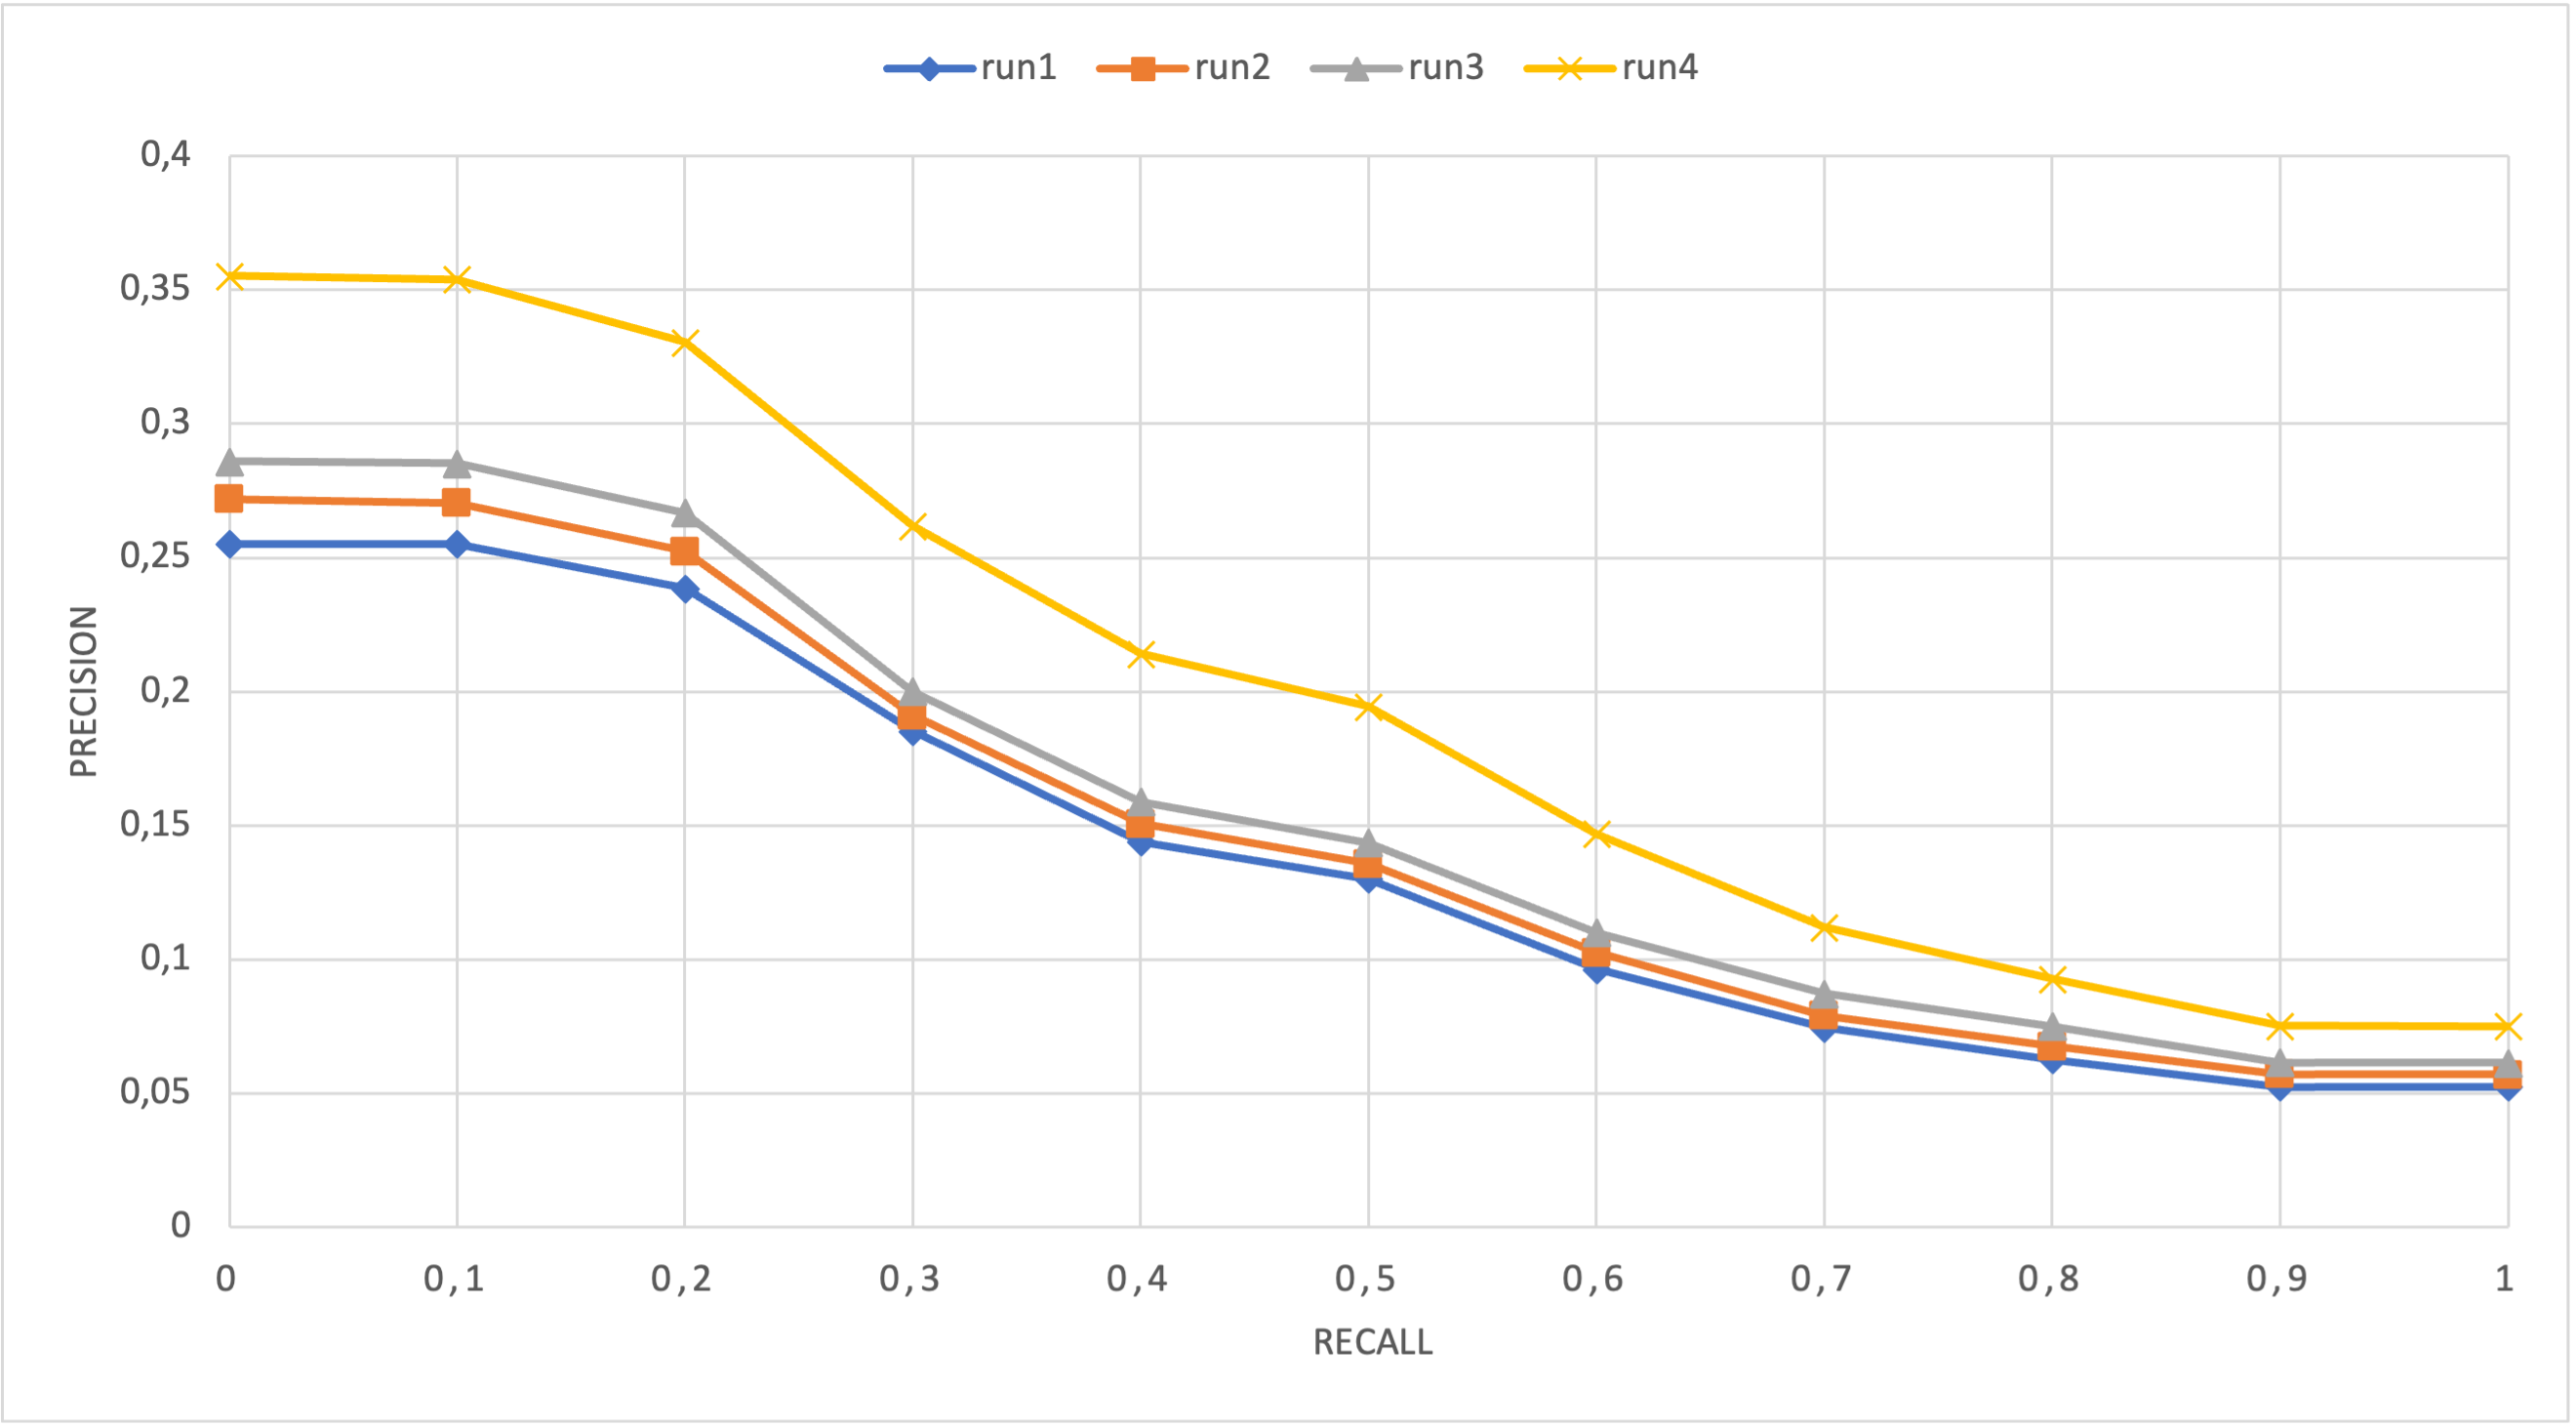
\includegraphics[width=\textwidth]{figure/rp_eng.png}
    \caption{Recall and precision graph}
    \label{fig:rp_english}
  \end{figure}